\documentclass[a4paper,titlepage,11pt]{article}

\usepackage[dutch]{babel}
\usepackage{graphicx}
\usepackage{ThemeJS}
\usepackage[defaultsans]{cantarell}
\renewcommand{\familydefault}{\sfdefault}
\usepackage[T1]{fontenc}

\title{Documentatie Project Memory Game}
\date{\today}
\author{Jan Hoekstra}

\def\myauthor{Jan Hoekstra} % Author
\def\mycoauthor{} % co-author
\def\mytitle{Documentatie Project} % title
\def\mysubtitle{Memory Game}
\def\mydate{\today} % date

\begin{document}
\pagenumbering{gobble}

\begin{titlepage}
\vspace{5cm}
\begin{tikzpicture}[remember picture, overlay]
  \path [left color = dark, bottom color = moderate, rotate=0] (current page.south west) rectangle (current page.north east);
\end{tikzpicture}

\centering
\vspace*{\fill}
\parbox[c][5cm][t]{10cm}{
  \color{white}\Huge\centering

  \mytitle \\
  \mysubtitle
  
  \vspace{3cm}
\huge
  \myauthor \\
  %\mycoauthor \\
  \mydate

}
\vspace*{\fill}

\end{titlepage}

\tableofcontents
%\clearpage
\pagenumbering{arabic}

\section{Voorwoord}

\subsection{Opdracht}

korte omschrijving opdracht

\subsection{Groep}

\begin{itemize}
\item Hoekstra, Jan Sietze
\item Meijer, Joost
\item Hooft, Emiel
\item Masselink, Tjibbe
\item Raven, Niek
\item B.A. Hensbergen \- Productowner
\end{itemize}

\clearpage

\section{Managementsamenvatting}

probleemschets, hoofdvraag, belang van de hoofdvraag
methode en werkwijze
resultaten
conclusies en aanbevelingen

\clearpage

\section{Inleiding}

\clearpage

\section{Projectomschrijving}

De bedoeling van dit project is het gaan opzetten van een Memory Game met de eisen en wensen van de klant. Het project wordt in een groep van 5 man groot uitgevoerd.

\subsection{Huidige situatie}

De projectgroep heeft de opdracht gekregen een memory spel te maken. Ze hebben toegang tot een tutor en een product owner voor hulp.

\subsection{Probleemstelling}

Er is behoefte aan een digitaal memory spel, ontwikkeld door de projectgroep. Zie [Eisen] voor alle verplichte eigenschappen van het memory spel.

\subsection{Werkwijze}

Voor het project is 1 periode vastgesteld. Week 1\-10 van het eerste schooljaar. De eerste 5 weken kunnen worden gebruikt voor planning etcetera en de 5 opvolgende weken voor het programmeren.

We gaan werken met een scrum methode, elke week een gedeelte. De eisen worden elke week opgesplitst. Elke week is er een demo voor de productowner.

\subsection{Definition of Done}

Een item is `done' wanneer:

\begin{itemize}

\item het door een teamgenoot gereviewed is
\item het getest is
\item het gedane werk omschreven staat in een user story
\item het gedocumenteerd is
\end{itemize}

\clearpage

\section{Functioneel Ontwerp}

\subsection{MoSCoW analyse}

{\bf Must Have}

\begin{itemize}
\item 4 x 4 matrix van kaarten
\item Gameveld moet dynamisch geladen worden
\item 2 Spelers moeten tegen elkaar kunnen spelen in 1 game
\item De spelers kunnen hun namen ingeven in het scherm;
\item Resetknop
\item Persistent scoreboard met namen met win/verlies status
\item Vanuit het hoofdmenu moet er genavigeerd kunnen worden naar een pagina waar de 
  highscores op te zien zijn
\item Status van spel bevriezen en later hervatten d.m.v. een tekstbestand
\end{itemize}

\noindent {\bf Should Have}
\begin{itemize}
\item Kaartenthema
\end{itemize}
\noindent {\bf Could Have}
\begin{itemize}
\item Spelers kunnen een avatar kiezen.
\end{itemize}
\noindent {\bf Won't have}
\begin{itemize}
\item Een optie in-game om kaartenthema te selecteren
\item Artificial Intelligence
\end{itemize}

\clearpage

\section{Technisch Ontwerp}

\subsection{Achtergrond}

\subsubsection{Te gebruiken technieken \& talen}

Om het memory project te realiseren worden de volgende technologieën gebruikt;
\begin{itemize}
\item Het project wordt geschreven in C\# en XAML
\item Er wordt gebruik gemaakt van Microsoft Visual Studio als ontwikkelomgeving
\item De widget toolkit die gebruikt wordt is Microsoft’s eigen Windows Presentation Foundation
\item Voor versiebeheer wordt gemaakt van Git in combinatie met GitHub
\end{itemize}

\subsection{Architectuur}

\subsubsection{Logica}

{\bf Waarom dit ontwerp}

Omdat de programmeurs nog niet veel ervaring hebben met ontwikkelen, laat staan
game state machines etc, wordt het ontwerp opzettelijk simpel gehouden.

{\bf Globaal}

De gamelogica wordt uitgevoerd in een loop. 
In het diagram hieronder is het belangrijkste gedeelte
van de high-level logica weergegeven. 

\begin{center}
\includegraphics[width=\linewidth]{../Images/diagram.png}
\end{center}

{\bf Gedetailleerd}

\begin{enumerate}
\item Matrix

De matrix wordt als een object aangemaakt. 
Dit object bevat alle benodigde informatie
voor het functioneren hiervan.

\item Kaarten
De kaarten worden als objecten aangemaakt. Deze objecten bevatten informatie zoals:

\begin{itemize}
\item Kaart ID (verwijst naar plaatje d.m.v. objectfunctie)
\end{itemize}
\end{enumerate}

\subsubsection{Opslaan/laden van savestates}

Omdat de matrix(incl. de kaarten) een object is,
kan dit makkelijk worden opgeslagen(geserialiseerd).
Variabelen kunnen ook makkelijk geserialiseerd worden.

\begin{center}
\includegraphics[width=.5\linewidth]{../Images/serialization.png}
\end{center}

\begin{center}
\includegraphics[width=.5\linewidth]{../Images/serialization2.png}
\end{center}

\subsubsection{User Interface}

De User Interface interactie wordt geabstraheerd doormiddel van een omkoepelende class.
Deze class is de enige route om wijzigingen in de UI uit te voeren.
Het voert geen gamelogica uit.

\subsection{Volgorde van onderdelen}

De volgorde waarin het programma wordt geschreven is:
\begin{enumerate}
\item 
\end{enumerate}

\subsection{Gemaakte keuzes architectuur}

In deze subsectie wordt omschreven welke keuzes tijdens het project zijn gemaakt,
deze zijn gedocumenteerd ter referentie.

\subsubsection{Logica}

{\bf Generatorfuncties:}
Om globale `state' te voorkomen, zijn zo veel mogelijk functies geschreven met
het doel een nieuw object terug te geven in plaats van een object van buiten te bewerken.

\subsubsection{Data}

{\bf Kaarten:}
De kaarten moeten worden opgeslagen in het programma,
bij voorkeur onafhankelijk van de gebruikersinterface.
Er is gekozen voor een 2D array met voor elke kaart een hashtable.


\begin{figure}[!hb]
  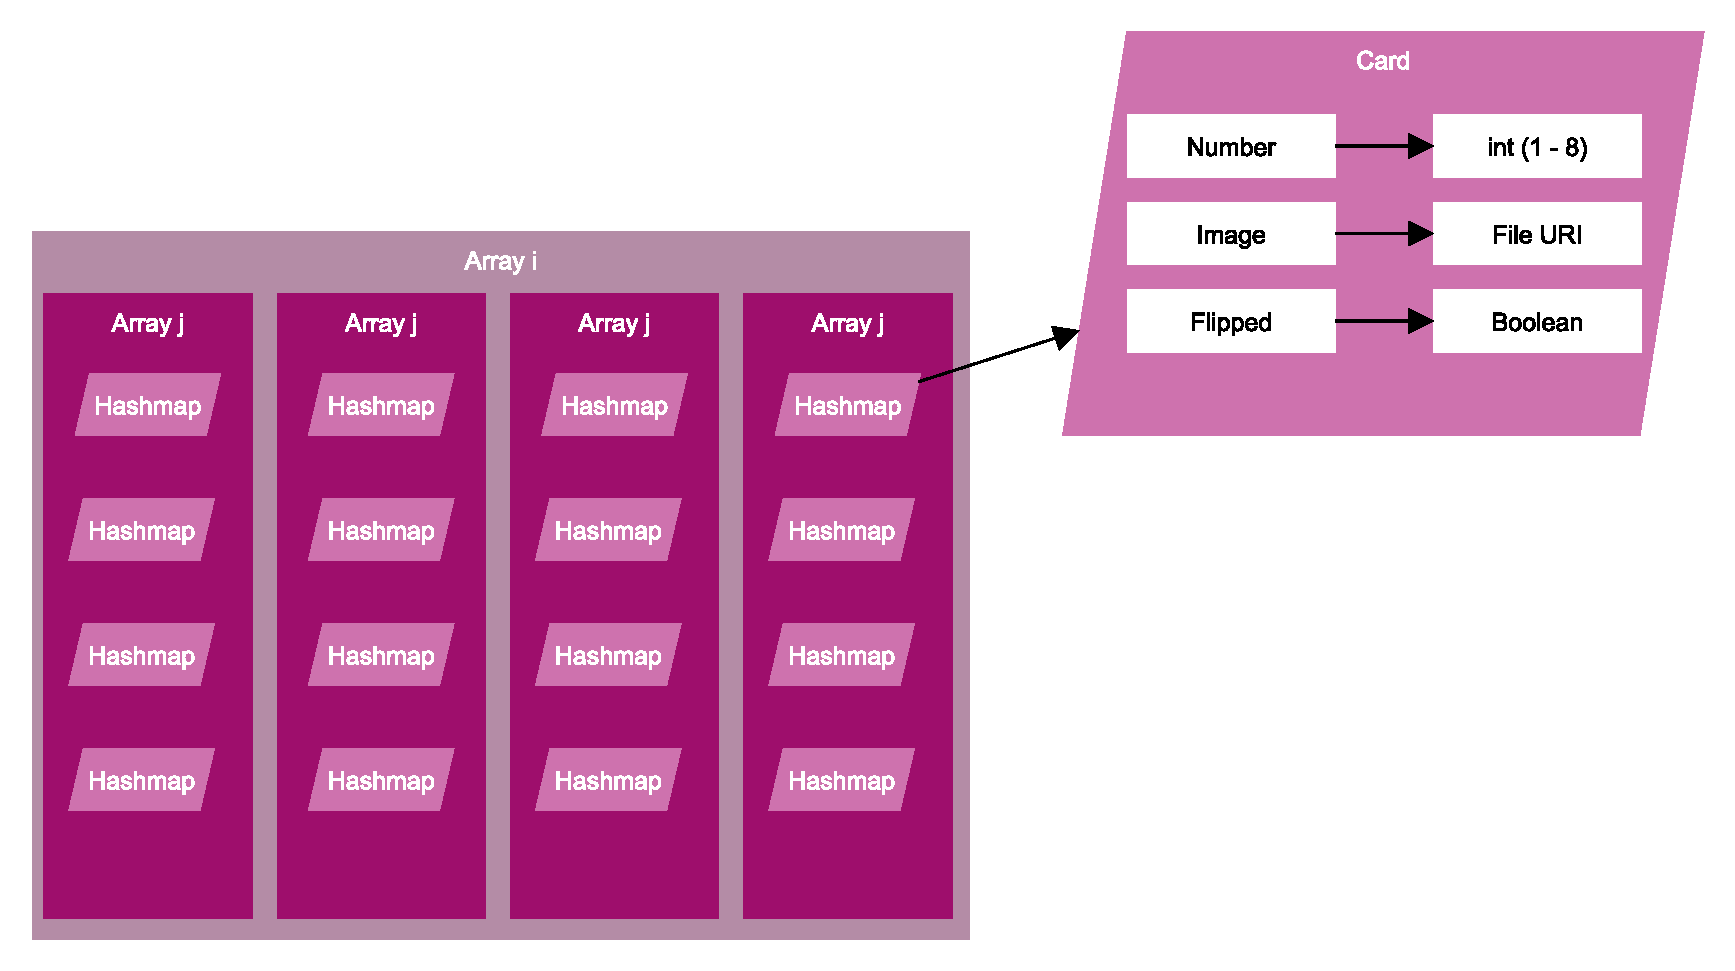
\includegraphics[width=\linewidth]{../Images/datastructure.pdf}
  \caption{Datastructuur}\label{fig:datastructure}
\end{figure}

\end{document}
